%%%%%%%%%%%%%%%%%%%%%%%%%%%%%%%%%%%%%%%%%%%%%%%%%%%%%%%%%%%%%%%%%%%%%%%%%%%%%%%%
%
% Template license:
% CC BY-NC-SA 3.0 (http://creativecommons.org/licenses/by-nc-sa/3.0/)
%
%%%%%%%%%%%%%%%%%%%%%%%%%%%%%%%%%%%%%%%%%%%%%%%%%%%%%%%%%%%%%%%%%%%%%%%%%%%%%%%%

%----------------------------------------------------------------------------------------
%	PACKAGES AND OTHER DOCUMENT CONFIGURATIONS
%----------------------------------------------------------------------------------------

\documentclass[
11pt, % The default document font size, options: 10pt, 11pt, 12pt
%oneside, % Two side (alternating margins) for binding by default, uncomment to switch to one side
%chapterinoneline,% Have the chapter title next to the number in one single line
spanish,
singlespacing, % Single line spacing, alternatives: onehalfspacing or doublespacing
%draft, % Uncomment to enable draft mode (no pictures, no links, overfull hboxes indicated)
%nolistspacing, % If the document is onehalfspacing or doublespacing, uncomment this to set spacing in lists to single
%liststotoc, % Uncomment to add the list of figures/tables/etc to the table of contents
%toctotoc, % Uncomment to add the main table of contents to the table of contents
parskip, % Uncomment to add space between paragraphs
%codirector, % Uncomment to add a codirector to the title page
headsepline, % Uncomment to get a line under the header
]{MastersDoctoralThesis} % The class file specifying the document structure



%----------------------------------------------------------------------------------------
%	INFORMACIÓN DE LA MEMORIA
%----------------------------------------------------------------------------------------

\thesistitle{People Behavior Tracking (PBT)} % El títulos de la memoria, se usa en la carátula y se puede usar el cualquier lugar del documento con el comando \ttitle

% Nombre del posgrado, se usa en la carátula y se puede usar el cualquier lugar del documento con el comando \degreename
%\posgrado{Carrera de Especialización en Sistemas Embebidos} 
%\posgrado{Carrera de Especialización en Internet de las Cosas} 
\posgrado{Carrera de Especialización en Inteligencia Artificial}
%\posgrado{Maestría en Sistemas Embebidos} 
%\posgrado{Maestría en Internet de las cosas}

\author{Ing. Hernán Contigiani} % Tu nombre, se usa en la carátula y se puede usar el cualquier lugar del documento con el comando \authorname

\director{PhD. Pasquinell Urbani (UCh - Globant S.A.)} % El nombre del director, se usa en la carátula y se puede usar el cualquier lugar del documento con el comando \dirname
\codirector{Nombre del codirector (pertenencia)} % El nombre del codirector si lo hubiera, se usa en la carátula y se puede usar el cualquier lugar del documento con el comando \codirname.  Para activar este campo se debe descomentar la opción "codirector" en el comando \documentclass, línea 23.

\juradoUNO{Esp. Ing. Juan Vicente Montilla Cabrera (FIUBA)} % Nombre y pertenencia del un jurado se usa en la carátula y se puede usar el cualquier lugar del documento con el comando \jur1name
\juradoDOS{Dr. Facundo Lucianna (FACET - UNT)} % Nombre y pertenencia del un jurado se usa en la carátula y se puede usar el cualquier lugar del documento con el comando \jur2name
\juradoTRES{Mg. Lic. Roberto Compañy (UCH)} % Nombre y pertenencia del un jurado se usa en la carátula y se puede usar el cualquier lugar del documento con el comando \jur3name

\ciudad{Ciudad Autónoma de Buenos Aires}
%\ciudad{ciudad de Mendoza}

\fechaINICIO{diciembre de 2020}
\fechaFINAL{agosto de 2021}


\keywords{Inteligencia artificial, visión por computadora} % Keywords for your thesis, print it elsewhere with \keywordnames


\begin{document}


\frontmatter % Use roman page numbering style (i, ii, iii, iv...) for the pre-content pages

\pagestyle{plain} % Default to the plain heading style until the thesis style is called for the body content


%----------------------------------------------------------------------------------------
%	RESUMEN - ABSTRACT 
%----------------------------------------------------------------------------------------

\begin{abstract}
\addchaptertocentry{\abstractname} % Add the abstract to the table of contents
%
%The Thesis Abstract is written here (and usually kept to just this page). The page is kept centered vertically so can expand into the blank space above the title too\ldots
\centering

La presente memoria describe el diseño de un sistema de monitoreo de personas desarrollado para Globant S.A. Tiene como principal objetivo estudiar los movimientos que realiza una persona al ingresar y transitar un espacio a fin de obtener métricas sobre las zonas que visitó.

Para poder realizar este trabajo se aplicaron conceptos de visión por computadora y aprendizaje profundo para detectar y seguir objetos en imágenes. Asimismo, se utilizaron técnicas de aprendizaje automático y segmentación para poder extraer características de dichos objetos con el propósito de aplicar técnicas de re-identificación y manejo de oclusiones que mejoran el seguimiento.

\end{abstract}

%----------------------------------------------------------------------------------------
%	CONTENIDO DE LA MEMORIA  - AGRADECIMIENTOS
%----------------------------------------------------------------------------------------

\begin{acknowledgements}
%\addchaptertocentry{\acknowledgementname} % Descomentando esta línea se puede agregar los agradecimientos al índice
\vspace{1.5cm}

A mi pareja, que me ha brindado su apoyo con cada nuevo desafío.

A mis compañeros y profesores, por compartir sus conocimientos y por su acompañamiento a lo largo de toda la carrera.

A mi director de proyecto, Pasquinell Urbani, por su orientación, seguimiento y aportes durante la realización del presente trabajo.

A todos ellos, muchas gracias.

\end{acknowledgements}

%----------------------------------------------------------------------------------------
%	LISTA DE CONTENIDOS/FIGURAS/TABLAS
%----------------------------------------------------------------------------------------

\tableofcontents % Prints the main table of contents

\listoffigures % Prints the list of figures

\listoftables % Prints the list of tables


%----------------------------------------------------------------------------------------
%	CONTENIDO DE LA MEMORIA  - DEDICATORIA
%----------------------------------------------------------------------------------------

%\dedicatory{\textbf{Dedicado a... [OPCIONAL]}}  % escribir acá si se desea una dedicatoria

%----------------------------------------------------------------------------------------
%	CONTENIDO DE LA MEMORIA  - CAPÍTULOS
%----------------------------------------------------------------------------------------

\mainmatter % Begin numeric (1,2,3...) page numbering

\pagestyle{thesis} % Return the page headers back to the "thesis" style

% Incluir los capítulos como archivos separados desde la carpeta Chapters

% Chapter 1

\chapter{Introducción general} % Main chapter title

\label{Chapter1} % For referencing the chapter elsewhere, use \ref{Chapter1} 
\label{IntroGeneral}

En este capítulo se realiza una introducción a los sistemas de monitoreo por visión artificial. Asimismo, se menciona el estado del arte de las tecnologías empleadas, y por último se explica la motivación, alcance y objetivos del presente trabajo.

%----------------------------------------------------------------------------------------
%	SECTION 1
%----------------------------------------------------------------------------------------

\section{Sistemas de monitoreo por visión}
\label{sec:sistemasVision}

En esta sección se introducen los sistemas de monitoreo por visión, las principales disciplinas de visión artificial y su utilización en el mercado.

\subsection{Visión artificial en la industria}

Los sistemas de visión artificial se basan en sensores digitales o cámaras que capturan imágenes para luego procesarlas y analizarlas. El sistema de software que analiza las imágenes utiliza técnicas de visión por computadora y/o aprendizaje profundo para extraer características. En la figura \ref{fig:visionArtificial} se observa un ejemplo del uso de visión artificial en una línea de producción, en la cual el brazo robot captura o selecciona determinados objectos en la línea que el sistema de visión encuentra y localiza.

\begin{figure}[ht]
	\centering
	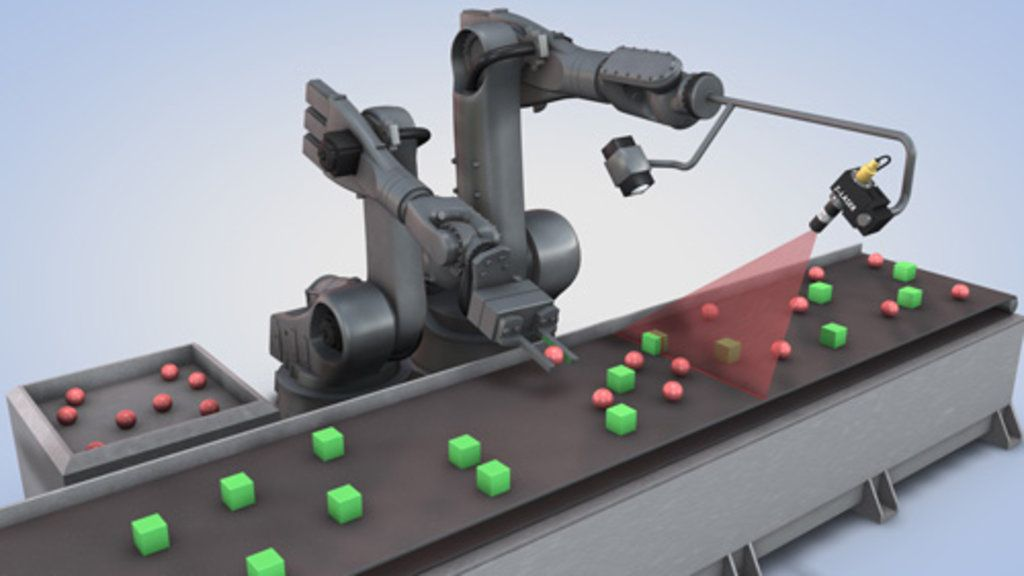
\includegraphics[scale=.55]{./Figures/visionArtificial.jpg}
	\caption{Utilización de visión artificial en la industria\protect\footnotemark.}
	\label{fig:visionArtificial}
\end{figure}

\footnotetext{Imagen tomada de \url{https://www.z-laser.es/aplicaciones/robotica.html}}

\newpage

Los sistemas de visión artificial se utilizan actualmente en diferentes ámbitos o industrias, como por ejemplo:
\begin{itemize}
\item En metrología: lo que hasta ahora se venía realizando con complejos equipos de metrología láser, se puede medir utilizando la visión artificial.
\item Detección de intrusos: se utiliza visión artificial para separar objectos no deseados en una línea transportadora, por ejemplo, remover ramas de una línea transportadora de frutas.
\item Verificación de montaje: se utiliza visión artificial para verificar el correcto montaje de un equipo o garantizar que no haya faltantes en una línea de montaje.
\item Sector médico: se utiliza visión artificial para apoyar al profesional médico y simplificar procesos de análisis de células cancerígenas, lunares y radiografías.
\item Sector automotriz: se utiliza visión artificial como un sistema que monitorea el tránsito y las condiciones de manejo, con el objetivo de evitar o reducir accidentes actuando en conjunto con otros sistemas de seguridad.
\end{itemize}

\subsection{Visión por computadora}

La visión artificial o visión por computadora \textit{(computer vision)} \citep{COMPUTER_VISION} es una rama de la ciencia de la computación que desarrolla métodos para adquirir, procesar y analizar imágenes del mundo real, con el fin de que una máquina pueda interpretarlas. Esta disciplina implementa herramientas de detección de patrones (líneas, bordes, texturas) llamadas filtros digitales. En la figura \ref{fig:visionComputadora} se observa un ejemplo del uso del ``algoritmo de Canny'' para la detecciones de bordes en una imagen.

\begin{figure}[ht]
	\centering
	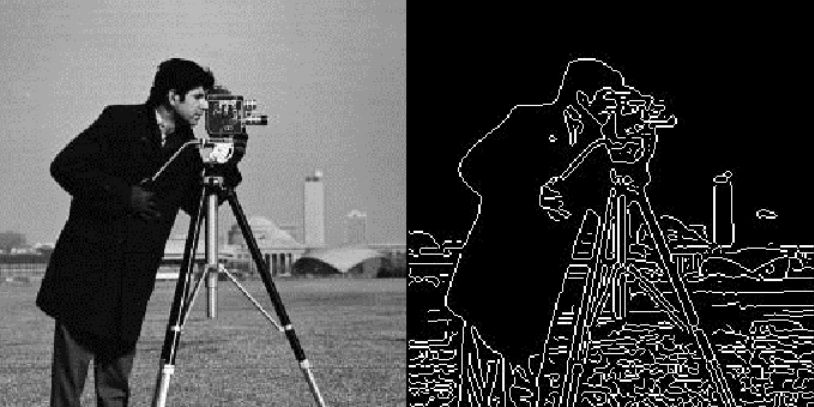
\includegraphics[scale=.55]{./Figures/visionComputadora.jpg}
	\caption{Filtro de Canny de visión por computadora\protect\footnotemark.}
	\label{fig:visionComputadora}
\end{figure}


\footnotetext{Imagen tomada de \url{https://www.researchgate.net/figure/The-Canny-Edger-on-the-image-Cameraman_fig13_266832526}}


Hasta principios de la década del 2010, los filtros clásicos de visión por computadora eran las herramientas más populares para analizar imágenes en la industria. En el 2012, con los primeros modelos de aprendizaje profundo para visión, la forma en la cual se trabaja y analiza las imágenes cambió drásticamente, abriendo un nuevo mundo de técnicas y posibilidades a la industria.

\newpage

\subsection{Aprendizaje profundo}

El aprendizaje profundo o \textit{Deep Learning} \citep{DEEP_LEARNING} es un subcampo de la inteligencia artificial, el cual utiliza distintas estructuras de redes neuronales para lograr representaciones de los datos cada vez más significativas. Las redes neuronales son un modelo computacional basado en un gran conjunto de unidades neuronales simples (neuronas artificiales), inspirado en el comportamiento observado de las neuronas en los cerebros humanos. 

Las técnicas de aprendizaje profundo combinadas con las técnicas de visión por computadora crearon las redes convolucionales. La arquitectura actual de redes convolucionales creada en 2012 revolucionó el campo del análisis de imágenes y video. En la figura \ref{fig:visionDeepLearning} se observan algunas de las técnicas de visión por aprendizaje profundo más populares, entre las que se encuentran: clasificación, detección y segmentación de imágenes.

\begin{figure}[ht]
	\centering
	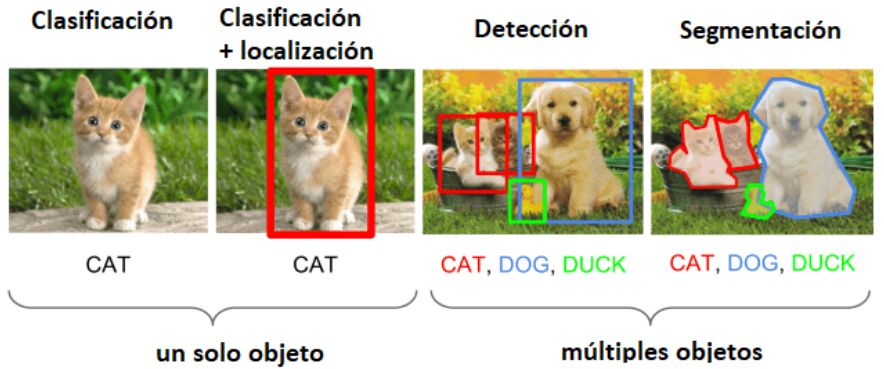
\includegraphics[scale=.7]{./Figures/visionDeepLearning.jpg}
	\caption{Técnicas de redes convolucionales en aprendizaje profundo\protect\footnotemark.}
	\label{fig:visionDeepLearning}
\end{figure}

\footnotetext{Imagen tomada de \url{https://ml4a.github.io/ml4a/convnets/}}

%----------------------------------------------------------------------------------------
%	SECTION 2
%----------------------------------------------------------------------------------------

\section{Motivación}
\label{sec:motivacion}

Una de las principales motivaciones en la realización de este trabajo es la adopción de las nuevas tecnologías de aprendizaje profundo en la industria y el  creciente desarrollo de estas. La incorporación de estas nuevas tecnologías permiten crear soluciones para monitorear condiciones en ambientes más adversos , como es el monitoreo de personas en una tienda.

Es notorio que a partir de la la década del 2010, la mayor cantidad de documentos científicos en el ámbito de la ciencia de la computación están enfocados en inteligencia artificial, que supera por mucho la cantidad de publicaciones de las otras ramas de esta ciencia \citep{AI_PAPERS}. El creciente desarrollo de la inteligencia artificial y su incorporación en la industria es posible gracias al avance del hardware, que hace posible ejecutar software más complejo, en tiempo real, pudiendo crear nuevas soluciones.

\newpage

En la figura \ref{fig:cpuGPU} se observa como han evolucionado las unidades de procesamiento gráfico (GPU) que hicieron posible esta nueva ola de desarrollo en el campo de la inteligencia artificial.

\begin{figure}[ht]
	\centering
	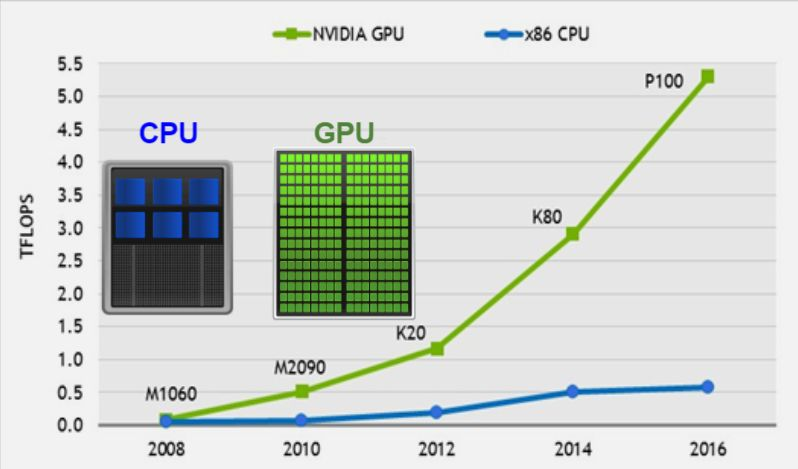
\includegraphics[scale=.8]{./Figures/cpuGPU.jpg}
	\caption{Evolución de las GPUs y CPUs\protect\footnotemark.}
	\label{fig:cpuGPU}
\end{figure}

\footnotetext{Imagen tomada de \url{https://www.networld.co.jp/files/9615/0846/8069/GPUs_Data_Analytics_Book.pdf}}

En el gráfico se compara la cantidad de operaciones de punto flotante por segundo (TFLOPS) \citep{TFLOPS} que pueden efectuar las GPUs y CPUs más modernas. Actualmente, una GPU puede contener 200 veces más núcleos que una CPU, permitiendo lograr más operaciones matemáticas simples por segundo. Los algoritmos de aprendizaje profundo se desarrollaron pensando en las operaciones que puede ejecutar y paralizar las GPUs, permitiendo que ejecutar algoritmos en tiempo real.

El creciente desarrollo de la inteligencia artificial viene acompañado por el fenómeno de ``big data''. Actualmente, la cantidad de información que se produce supera la cantidad de información generada en toda la historia de la humanidad. Esto es posible ya que todas las personas están interactuando constantemente con la nube mediante dispositivos conectados a internet (redes sociales, foros, juegos). A todo este ecosistema se suma internet de las cosas (IoT), en donde los dispositivos (sensores, computadoras, cámaras) recolectan y suben información constantemente a la nube para el monitoreo y control de sistemas, casas y productos.

\newpage

%----------------------------------------------------------------------------------------
%	SECTION 3
%----------------------------------------------------------------------------------------

\section{Estado del arte}
\label{sec:estadoDelArte}

Los sistemas de monitoreo de objectos por visión incorporan una serie de técnicas y modelos de inteligencia artificial, que juntos en una cadena de procesamiento, permiten detectar y seguir diferentes clases de objectos en una imagen o video. Estas técnicas no requieren utilizar cámaras de alta resolución, y pueden llegar a ejecutarse dentro de un dispositivo embebido o un celular. Las técnicas de aprendizaje profundo involucradas en estos sistemas son:

\begin{itemize}
\item Detección de objetos en imágenes: se utilizan modelos de inteligencia artificial que localizan objectos de interés en imágenes. Según la precisión deseada y el poder de computo del dispositivo será el modelo detector que se utilice en el sistema.
\item Seguir objectos en imágenes: se utilizan modelos de inteligencia artificial que consumen las detecciones del modelo anterior, y permiten seguir la trayectoria de los objectos en una imagen o video.
\end{itemize}

Estas técnicas y modelos de inteligencia artificial se pueden acceder de forma pública para su uso académico o comercial. La dificultad que existe actualmente en estos sistemas de monitoreo son los desafíos que se detallan en la sección \ref{sec:desafiosSeguimiento}, los cuales se abordan en este trabajo.

%----------------------------------------------------------------------------------------
%	SECTION 4
%----------------------------------------------------------------------------------------

\section{Objetivos y alcance}
\label{sec:objetivosAlcance}

\subsection{Objetivos}

El propósito de este trabajo fué el desarrollo de un sistema de monitoreo de personas. Tiene como principal objetivo estudiar los movimientos que realiza un individuo al ingresar y transitar un espacio a fin de obtener métricas sobre las zonas que visitó. Para poder cumplir este objetivo es necesario poder detectar a las personas que aparecen en el video tomado por una cámara, realizar el seguimiento de cada una y poder identificarlas aún cuando desaparecen del espacio de visión por unos segundos.

En la figura \ref{fig:esquemaGeneral} se observa un diagrama general de la solución y las etapas que la componen.

\begin{figure}[ht]
	\centering
	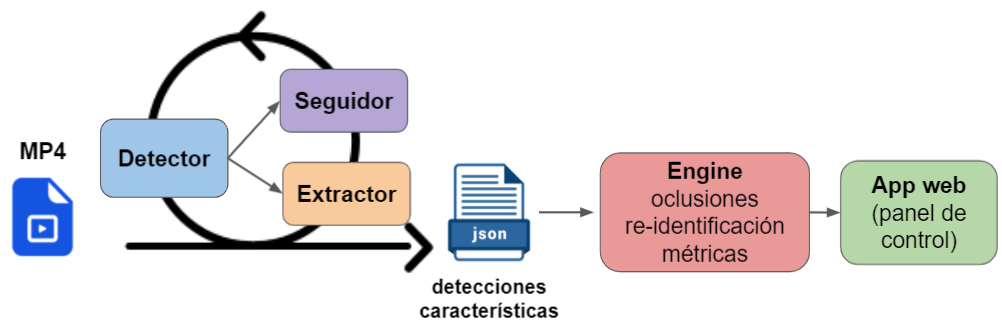
\includegraphics[scale=.6]{./Figures/esquemaGeneral.png}
	\caption{Diagrama general de la solución.}
	\label{fig:esquemaGeneral}
\end{figure}

\newpage

\subsection{Alcance}

Para la elaboración de este trabajo, la parte del sistema involucrada con aprendizaje profundo (el detector, seguidor y extractor) se ejecutó en una plataforma que proporciona una GPU para la ejecución de los modelos. La otra parte del sistema, el ``Engine'' y la aplicación web, se ejecutaron en una máquina personal. El desarrollo de las etapas mencionadas incluye los siguientes aspectos:
\begin{itemize}
\item Implementación de una cadena de procesamiento de inteligencia artificial que consuma videos \file{.mp4} y detecte personas.
\item Implementación de un sistema de mejora de monitoreo (``Engine''), que aborde los problemas de oclusiones y re-identificación de personas.
\item Implementación de una aplicación web para la configuración general del sistema.
\item Visualización de los datos en tiempo real en la aplicación web.
\item Alcanzar los requerimientos de monitoreo de personas establecidos en la sección \ref{sec:requerimientos}.
\end{itemize}



\chapter{Introducción específica} % Main chapter title

\label{Chapter2}

En este capítulo

%----------------------------------------------------------------------------------------
%	SECTION 1
%----------------------------------------------------------------------------------------

\section{Requerimientos}
\label{sec:requerimientos}

Es esta sección

\subsection{Tablas}

Para las tablas utilizar el mismo formato que para las figuras, sólo que el epígrafe se debe colocar arriba de la tabla, como se ilustra en la tabla \ref{tab:peces}. Observar que sólo algunas filas van con líneas visibles y notar el uso de las negritas para los encabezados.  La referencia se logra utilizando el comando \verb|\ref{<label>}| donde label debe estar definida dentro del entorno de la tabla.

\begin{verbatim}
\begin{table}[h]
	\centering
	\caption[caption corto]{caption largo más descriptivo}
	\begin{tabular}{l c c}    
		\toprule
		\textbf{Especie}     & \textbf{Tamaño} & \textbf{Valor}\\
		\midrule
		Amphiprion Ocellaris & 10 cm           & \$ 6.000 \\		
		Hepatus Blue Tang    & 15 cm           & \$ 7.000 \\
		Zebrasoma Xanthurus  & 12 cm           & \$ 6.800 \\
		\bottomrule
		\hline
	\end{tabular}
	\label{tab:peces}
\end{table}
\end{verbatim}

%----------------------------------------------------------------------------------------
%	SECTION 2
%----------------------------------------------------------------------------------------

\section{Modelos de inteligencia artificial utilizados}
\label{sec:requerimientos}

\subsection{Detector Yolo}

\textit{Yolo (You Only Look once)}\footnote{\url{https://en.wikipedia.org/wiki/Raster_graphics}} es un detector...


\begin{figure}[ht]
	\centering
	\includegraphics[scale=.50]{./Figures/questionMark.png}
	\caption{Esquema de funcionamiento de Yolo.}
	\label{fig:diagramaYolo}
\end{figure}



\subsection{Seguidor Deepsort}

\subsection{Extractor de características Osnet}

%----------------------------------------------------------------------------------------
%	SECTION 3
%----------------------------------------------------------------------------------------

\section{Desafíos en el seguimiento de personas}
\label{sec:desafiosSeguimiento}

%----------------------------------------------------------------------------------------
%	SECTION 4
%----------------------------------------------------------------------------------------

\section{Zonas de interés}
\label{sec:zonasInteres}
 
\chapter{Diseño e implementación} % Main chapter title

\label{Chapter3} % Change X to a consecutive number; for referencing this chapter elsewhere, use \ref{ChapterX}

En este capítulo

%----------------------------------------------------------------------------------------
%	SECTION 1
%----------------------------------------------------------------------------------------

\section{Cadena de procesamiento de inteligencia artificial}
\label{sec:cadenaProcesamiento}

\subsection{Arquitectura}

\subsection{Integración de los modelos}

%----------------------------------------------------------------------------------------
%	SECTION 2
%----------------------------------------------------------------------------------------

\section{Entrenamiento de un modelo basado en Osnet}
\label{sec:entrenamientoOsnet}

\subsection{Preparación de datos}

\subsection{Entrenamiento grueso y fino}

\subsection{Comparativa de los diferentes modelos de extracción de características}

%----------------------------------------------------------------------------------------
%	SECTION 3
%----------------------------------------------------------------------------------------

\section{Manejo de oclusiones y re-identificación}
\label{sec:oclusionesReID}

\subsection{Segmentación de personas}

\subsection{Re-identificación por vectores}

\subsection{Mejora del seguimiento por vectores}

\subsection{Validación del manejo de oclusiones y re-identificación}

%----------------------------------------------------------------------------------------
%	SECTION 4
%----------------------------------------------------------------------------------------

\section{Motor de seguimiento y monitoreo (Engine)}
\label{sec:engine}

\subsection{Arquitectura}

\subsection{Máquina de estados}

%----------------------------------------------------------------------------------------
%	SECTION 5
%----------------------------------------------------------------------------------------

\section{Interfaz de usuario}
\label{sec:gui}

\subsection{Definición de zonas de interés}

\subsection{Visualización del seguimiento}

\subsection{Visualización de las métricas}


% Chapter Template

\chapter{Ensayos y resultados} % Main chapter title

\label{Chapter4} % Change X to a consecutive number; for referencing this chapter elsewhere, use \ref{ChapterX}

En este capítulo se detallan los resultados esperados y obtenidos sobre cada etapa del trabajo. A su vez, se indican las herramientas y metodologías empleadas en cada caso. Finalmente se expone el caso de uso completo integrando todos los componentes que integran al sistema.

%----------------------------------------------------------------------------------------
%	SECTION 1
%----------------------------------------------------------------------------------------

\section{Descripción del banco de pruebas}
\label{sec:bancoPruebas}

Para poder evaluar la detección, el seguimiento y la re-identificación de personas, se somete al sistema a una validación visual a partir del análisis de los videos procesados por cada parte del sistema. El sistema se evalúa en las siguientes etapas:

\begin{itemize}
\item Modelos de detección y seguimientos de personas.
\item Extractor de características.
\item Manejo de oclusiones y re-identificación de personas.
\end{itemize}

En la sección \ref{sec:validDetectorSeguidor} se detallan los criterios de validación empleados para evaluar los videos generados que se pueden observar en la figura \ref{fig:bancoPruebas}.

\begin{figure}[ht]
	\centering
	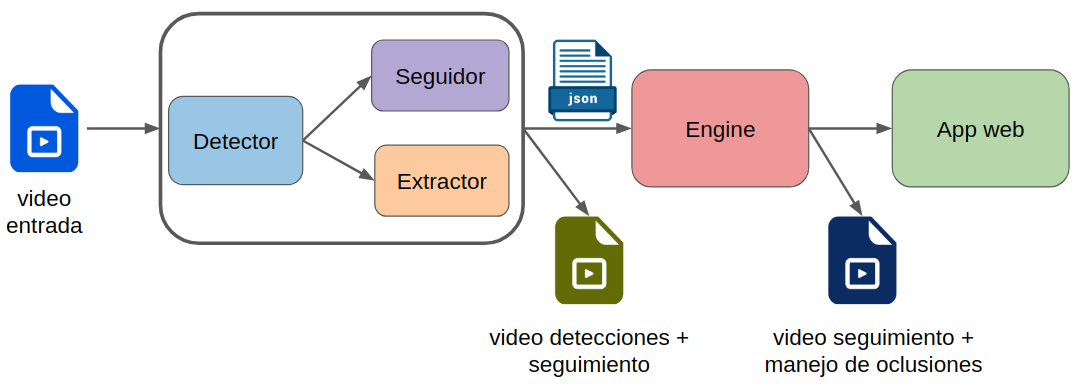
\includegraphics[scale=.50]{./Figures/bancoPruebas.png}
	\caption{Videos de ensayo generados en cada etapa.}
	\label{fig:bancoPruebas}
\end{figure}



Para poder evaluar la calidad del extractor de características, se creó un programa que facilita la captura de imágenes de personas en un video. En la figura \ref{fig:imagenesCrop} se pueden observar ejemplos de capturas realizadas de una misma persona en diferentes poses y locaciones a fin de generar un pequeño banco de imágenes de cada individuo. En la sección \ref{sec:validExtractor} se detallan los criterios de validación empleados para evaluar el extractor a partir del uso de estas imágenes.

\newpage

\begin{figure}[ht]
	\centering
	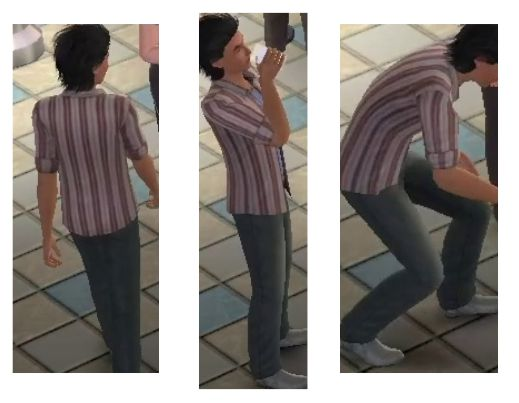
\includegraphics[scale=.45]{./Figures/imagenesCrop.jpg}
	\caption{Capturas tomadas de una persona.}
	\label{fig:imagenesCrop}
\end{figure}

De la experiencia obtenida de evaluar videos y el extractor de características, se desarrolló un programa capaz de automatizar los ensayos de validación del sistema. En la sección \ref{sec:precisionSistema} se detalla como se utilizó este programa para obtener métricas automáticas de la precisión de cada etapa y del sistema global.

%\newpage

%----------------------------------------------------------------------------------------
%	SECTION 2
%----------------------------------------------------------------------------------------

\section{Validación de los modelos de detección y seguimiento}
\label{sec:validDetectorSeguidor}

Validar sistemas de monitoreo por visión o procesamiento de imágenes normalmente implica una inspección manual por parte de un experto (conocedor del sistema y los objetivos a lograr) ya que es un proceso muy complejo de automatizar. El proceso empleado consiste en:

\begin{itemize}
\item Analizar si hay una zona de la cámara en donde las personas no están siendo detectadas.
\item Analizar si hay problemas de iluminación o de foco en los videos capturados.
\item Evaluar si las detecciones son continuas, o si las personas están constantemente cambiando de estado de detectada a no detectada.
\item Evaluar si hay falsos positivos, es decir, objetos que no son personas detectadas en el video.
\item Evaluar si el seguidor mantiene el mismo identificador para cada persona a medida que transitan por el recinto.
\item Detectar posibles oclusiones estáticas en el recinto que perjudiquen al sistema (por ejemplo un cartel que tape a las personas).
\item Evaluar con que frecuencia ocurre alguno de los desafíos conocidos en el seguimiento de cada persona (oclusiones, pérdidas o cambios de identificadores, personas que salen y vuelven a ingresar a cámara).
\end{itemize}

En la figura \ref{fig:fallasDetector} se pueden observar ejemplos de problemas que ocurren con el detector que precisan examinación manual.

%La figura \ref{fig:fallasDetector1de3}, \ref{fig:fallasDetector2de3} y \ref{fig:fallasDetector3de3}.

\newpage

\begin{figure}[!htpb]
     \centering
     \begin{subfigure}[b]{0.3\textwidth}
         \centering
         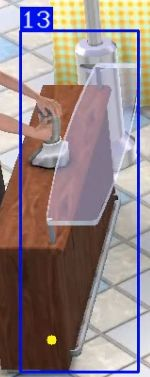
\includegraphics[width=.65\textwidth]{./Figures/fallasDetector1.jpg}
         \caption{Falsa detección.}
         \label{fig:fallasDetector1de3}
     \end{subfigure}
     \hfill
     \begin{subfigure}[b]{0.3\textwidth}
         \centering
         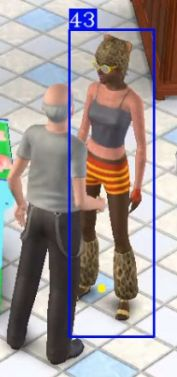
\includegraphics[width=.65\textwidth]{./Figures/fallasDetector2.jpg}
         \caption{No detección.}
         \label{fig:fallasDetector2de3}
     \end{subfigure}
     \hfill
     \begin{subfigure}[b]{0.3\textwidth}
         \centering
         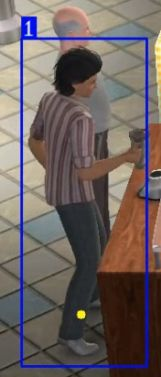
\includegraphics[width=.65\textwidth]{./Figures/fallasDetector3.jpg}
         \caption{Oclusión.}
         \label{fig:fallasDetector3de3}
     \end{subfigure}
        \caption{Fallas en la detección de personas.}
        \label{fig:fallasDetector}
\end{figure}

Es fundamental esta etapa de análisis porque permite entender las debilidades y fortalezas del sistema en una primera etapa de desarrollo.



%----------------------------------------------------------------------------------------
%	SECTION 3
%----------------------------------------------------------------------------------------

\section{Validación del modelo de extracción de características}
\label{sec:validExtractor}

Para evaluar la calidad del extractor de características no alcanzan las métricas de segmentación obtenidas en la sección \ref{sec:comparativaExtractores}. Es necesario llevar el concepto de re-identificación por vectores de características a algo tangible. Para ello, se creó un programa que permite realizar el seguimiento de personas únicamente por sus características, el cual se detalla en el diagrama de la figura \ref{fig:seguidorPorCaracteristicas}.

\begin{figure}[ht]
	\centering
	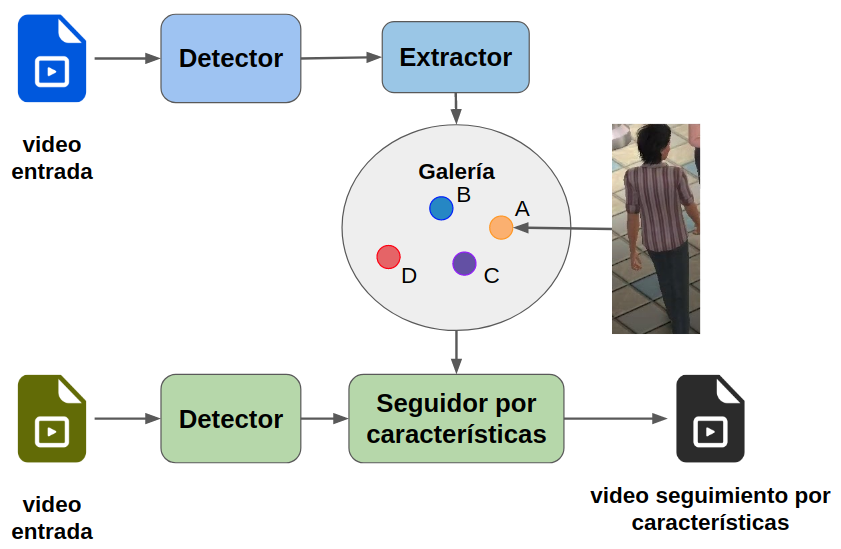
\includegraphics[scale=.60]{./Figures/seguidorPorCaracteristicas.png}
	\caption{Programa de seguimiento por características.}
	\label{fig:seguidorPorCaracteristicas}
\end{figure}

\newpage

El procedimiento llevado a cabo requiere dos iteraciones del video de entrada, en la primera se obtiene como salida la galería de características y en la segunda se obtiene el video de seguimiento por características.

Primera iteración del video:
\begin{itemize}
\item El sistema levanta las capturas de la imágenes de las personas y calcula los vectores de características de cada una.
\item Arma una galería de clusters de personas utilizando los vectores calculados.
\item Se analizan los clusters de la galería utilizando una herramienta que permite evaluarlos y graficarlos (ver figura \ref{fig:tsneClusers}).
\end{itemize}

\begin{figure}[ht]
	\centering
	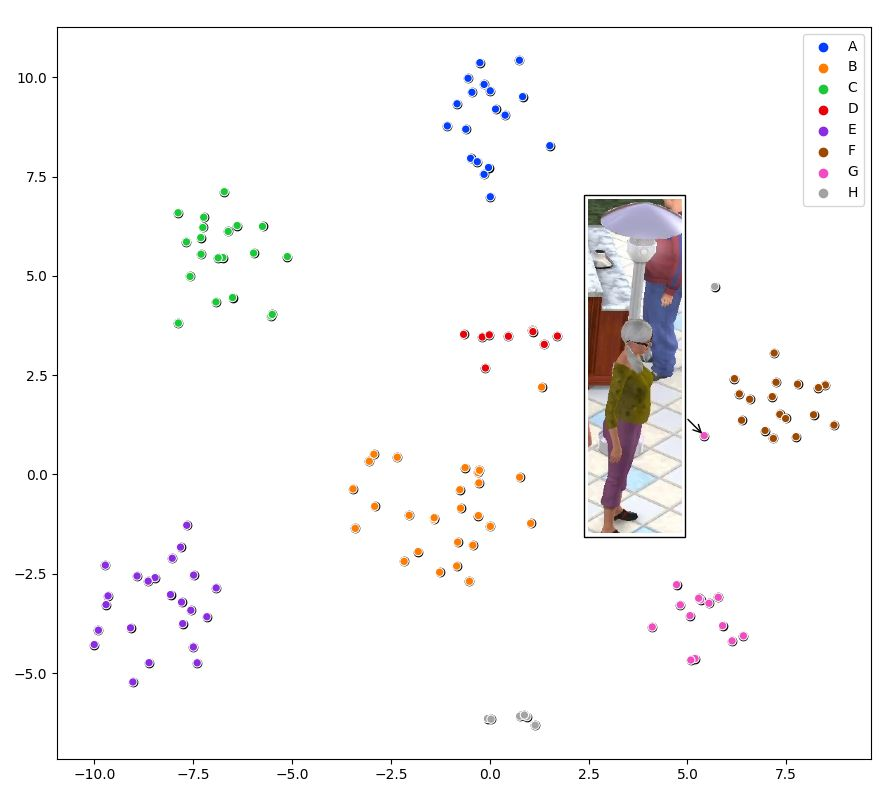
\includegraphics[scale=.60]{./Figures/tsneClusers.jpg}
	\caption{Análisis de los clusters generados.}
	\label{fig:tsneClusers}
\end{figure}

La herramienta para analizar clusters permite sacar conclusiones como las siguientes:
\begin{itemize}
\item No hay solapamiento de clusters en la galería y los clusters se encuentran bien separados.
\item Se puede observar que el cluster ``G'' tiene un vector muy cercano al cluster ``F'', debido a que dicho vector se calcula sobre una captura en donde ambas personas aparecen en la imagen.
\end{itemize}

\newpage

Segunda iteración del video:
\begin{itemize}
\item De cada detección reportada se extrae su vector de características.
\item El sistema toma cada vector de características y busca en la galería de clusters de personas a cual pertenece.
\item En caso de encontrar una persona candidata para esa detección, le asigna la letra de ese cluster.
\item Se genera un video de salida en donde las personas detectadas son representadas por las letras de los clusters candidatos.
\end{itemize}

La salida del sistema es un nuevo video con las detecciones de las personas. En vez de utilizar el seguidor para asignarles un identificador único a cada persona, se utiliza el procedimiento explicado en la figura \ref{fig:seguidorPorCaracteristicas} para asignar una letra a cada detección. En la figura \ref{fig:videoPorCaracteristicas} se observa un ejemplo del video resultante.

\begin{figure}[ht]
	\centering
	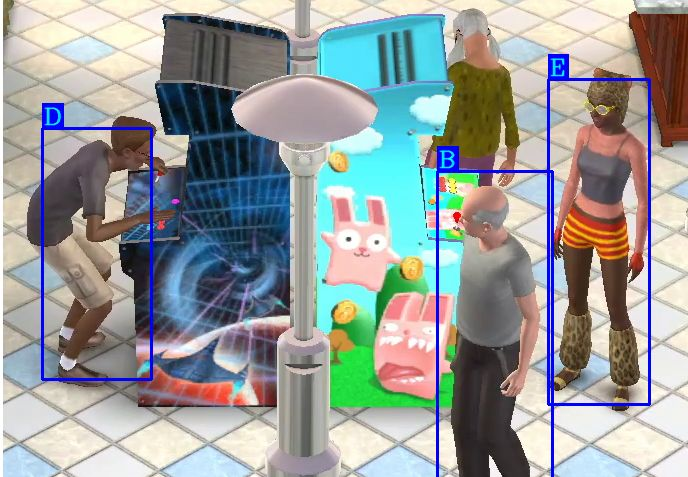
\includegraphics[scale=.60]{./Figures/videoPorCaracteristicas.jpg}
	\caption{Sistema de seguimiento por características.}
	\label{fig:videoPorCaracteristicas}
\end{figure}

Este proceso es muy robusto porque el sistema en la segunda iteración analiza el video conociendo de antemano las diferentes poses de cada persona, es decir, inicia el proceso con información futura. Las capturas de las personas se encuentran transformadas en clusters dentro de la galería. Por lo tanto, si la galería está correctamente armada se puede realizar seguimiento de personas por características sin errores. Utilizando este sistema se pueden obtener métricas automáticas de los videos obtenidos a la salida del Engine, por ejemplo:
\begin{itemize}
\item Cuánto tiempo fue monitoreada cada persona de forma correcta.
\item Cuántos identificadores distintos se asignaron a una misma persona.
\item Cuántos intercambios de identificadores hay en todo el video.
\end{itemize}

\newpage

%----------------------------------------------------------------------------------------
%	SECTION 4
%----------------------------------------------------------------------------------------

\section{Precisión de cada módulo del sistema}
\label{sec:precisionSistema}

Utilizando las métricas automáticas obtenidas en la sección \ref{sec:validExtractor} se puede validar por cada video procesado los siguientes requerimientos:
\begin{itemize}
\item Se considerará que una persona es correctamente monitoreada si al menos se mantuvo su seguimiento el 80\% del tiempo que circuló en el recinto.
\item Se considerará que el sistema funciona dentro de los parámetros aceptables si entre el 80\% y 100\% de las personas en el video fueron correctamente monitoreadas.
\end{itemize}

En la figura \ref{fig:metricasPorPersona} se observa el porcentaje de correcto seguimiento correspondiente a cada persona en el video luego de toda la cadena de procesamiento.

\begin{figure}[ht]
	\centering
	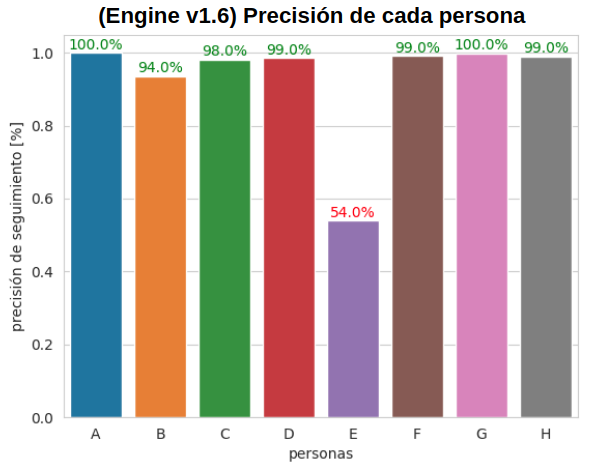
\includegraphics[scale=.80]{./Figures/metricasPorPersona.png}
	\caption{Precisión de seguimiento por persona.}
	\label{fig:metricasPorPersona}
\end{figure}

En la figura \ref{fig:metricasPorPersona} se observa que siete de ocho personas tienen una precisión de seguimiento por arriba del 80\%, y por lo tanto, la precisión total del sistema para ese video es de 87.5\%. 

En la figura \ref{fig:metricasPorSistema} se aplica la misma lógica para calcular la precisión de cada etapa del sistema y sus diferentes versiones para un mismo video de entrada.

\newpage

\begin{figure}[ht]
	\centering
	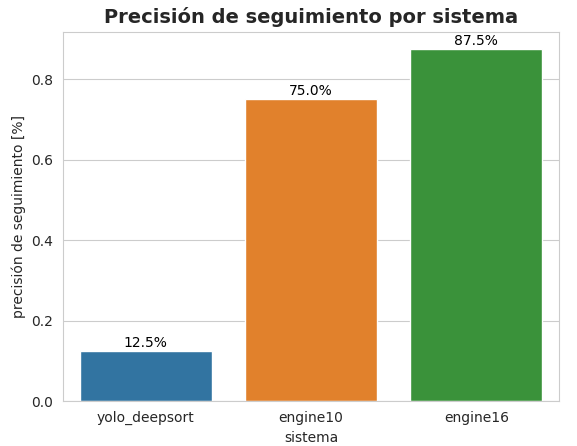
\includegraphics[scale=.80]{./Figures/metricasPorSistema.png}
	\caption{Precisión de seguimiento por sistema.}
	\label{fig:metricasPorSistema}
\end{figure}

Descripción de la evolución de los sistemas de la figura \ref{fig:metricasPorSistema}:
\begin{itemize}
\item Yolo y Deepsort: precisión que se alcanza si se utiliza el detector Yolo y el seguidor Deepsort tal cual se encuentra disponible en la web.
\item Engine10: precisión que se alcanza si al detector Yolo y al seguidor Deepsort se agrega el postprocesado del Engine v1.0 utilizando los vectores de características para el manejo de oclusiones y re-identificación de personas.
\item Engine16: precisión que se alcanza si al detector Yolo y al seguidor Deepsort se agrega el postprocesado del Engine v1.6 utilizando los vectores de características para el manejo de oclusiones y re-identificación de personas junto con la información agregada de las las zonas de interés.
\end{itemize}

En conclusión, la precisión del sistema aumenta con cada nueva funcionalidad que se incorpora. Por otro lado, en la figura \ref{fig:idSwitch} se observa que a medida que evolucionan los sistemas también se reducen los intercambios de identificador entre personas.

\newpage

\begin{figure}[ht]
	\centering
	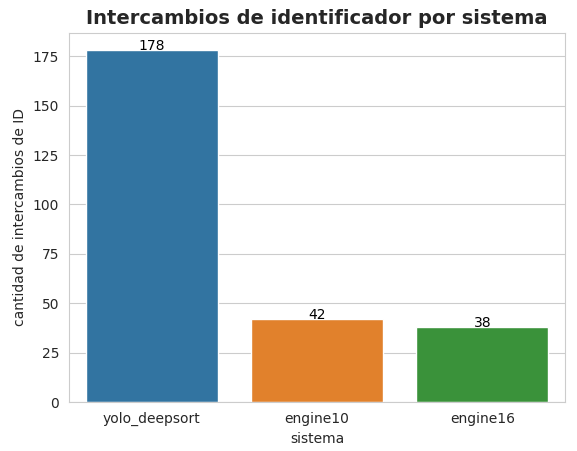
\includegraphics[scale=.80]{./Figures/idSwitch.png}
	\caption{Intercambios de identificador por sistema.}
	\label{fig:idSwitch}
\end{figure}

Con la última versión del Engine se logra alcanzar la precisión deseada de seguimiento, ya que con el agregado de las zonas se redujeron las falsas detecciones e intercambios de identificadores.

%----------------------------------------------------------------------------------------
%	SECTION 5
%----------------------------------------------------------------------------------------

\section{Simulaciones}
\label{sec:simulaciones}

Durante la realización de este trabajo no se tomaron muestras de videos de tiendas o recintos para realizar ensayos y validación, sino que se contó con el material de video disponible en internet. El problema es que la mayoría del material disponible es de muy corta duración (menor al minuto) o circulan muy pocas personas por el recinto (dos a tres personas). Debido a estos problemas fue muy difícil al comienzo validar las primeras etapas del trabajo.

El único video que se encontró en internet que cumpliera con todas las características fue un video de una tienda \citep{TIENDA_ORIGINAL} en donde aparecen más de 10 personas por más de un minuto. Este video se utilizó para las primeras demostraciones \citep{DEMO:1} con el fin de validar el sistema de re-identificación y manejo de oclusiones. El inconveniente con este video es que no resultó posible probar todas las funcionalidades de las zonas de interés. Principalmente, debido a que el espacio es bastante reducido y las personas durante la duración del video no llegan a transitar por más de una zona como se observa en la figura \ref{fig:tienda}.

\begin{figure}[ht]
	\centering
	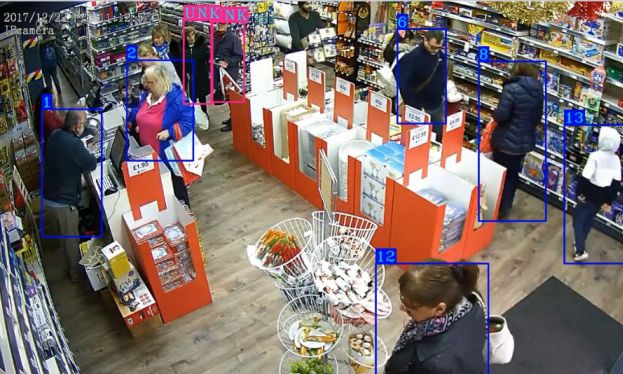
\includegraphics[scale=.70]{./Figures/tienda.jpg}
	\caption{Imagen del video de tienda utilizado al comienzo del trabajo.}
	\label{fig:tienda}
\end{figure}

\newpage

Dado que se necesitaba un video de un recinto con más zonas de interés y personas que se involucraran más con el espacio se buscó simular el entorno. Para ello, se optó por utilizar el videojuego ``Los Sims 3'' \citep{SIMS3}, en el cual es posible crear un ambiente totalmente a medida y personajes que interactúan en él. El juego permite crear personajes con diferentes personalidades por lo que cada uno interactúa de forma singular con el espacio pudiéndose obtener distintas métricas por el tiempo que se desee que dure el ensayo. En la figura \ref{fig:sims} se observa el entorno creado para ensayar las últimas funcionalidades creadas en el sistema, como por ejemplo las zonas de interés, las métricas y la aplicación web.

\begin{figure}[ht]
	\centering
	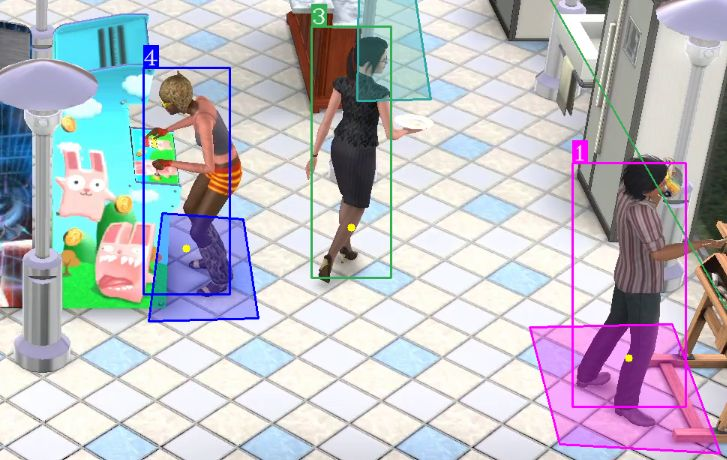
\includegraphics[scale=.50]{./Figures/sims.jpg}
	\caption{Imagen del escenario creado en el video juego ``Los Sims 3''.}
	\label{fig:sims}
\end{figure}

\newpage

El video generado a partir del simulador fue un éxito y permitió terminar de ensayar y validar todas las funcionalidades del sistema sin inconvenientes. En los primeros videos de simulación el detector apenas conseguía capturar a los personajes en el video, dado que la resolución de grabación y la calidad de las luces y sombras era baja. Se necesitó elaborar diez configuraciones diferentes de captura de video para que los colores y los personajes se vieran lo más realistas posible y el detector pudiera identificar a los personajes del juego como personas reales.

El resultado final \citep{DEMO:2} se acerca a un escenario real, ya que el detector presenta más inconvenientes detectando a los personajes que a las personas reales en la tienda y es por ello que la precisión de seguimiento utilizando solo el detector y seguidor para este video es muy baja. Finalmente, el video generado como una simulación pudo utilizarse luego de encontrar la configuración de video adecuada gracias a que el sistema de re-identificación ayuda a salvar todos los defectos del detector en el seguimiento de estos personajes ficticios.

%----------------------------------------------------------------------------------------
%	SECTION 5
%----------------------------------------------------------------------------------------

\section{Resultados}
\label{sec:resultados}

En esta sección se detallan los resultados y métricas obtenidas en la aplicación web luego de procesar el video de ``Los Sims'' con el Engine v1.6. En la aplicación web las detecciones y las personas se ejemplifican con figuras geométricas, ya que no se realiza la transmisión del video original en la misma; como se observa en la figura \ref{fig:simsWebApp}.

\begin{figure}[ht]
	\centering
	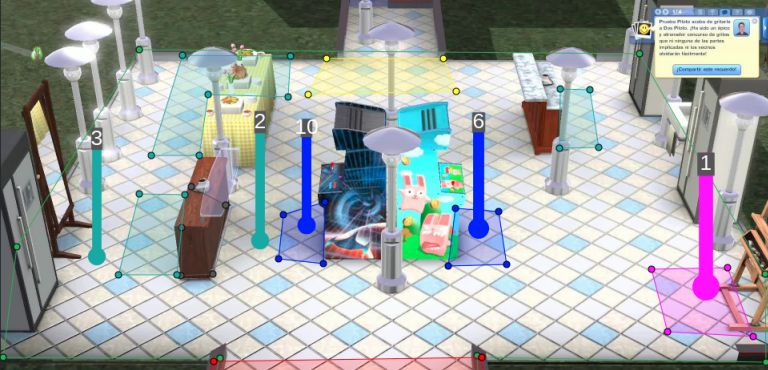
\includegraphics[scale=.60]{./Figures/simsWebApp.jpg}
	\caption{Imagen del monitoreo de personas en la aplicación web.}
	\label{fig:simsWebApp}
\end{figure}

Además de contar con el seguimiento y monitoreo de cada persona en la aplicación web, a la izquierda se cuenta con un panel que se actualiza en tiempo real en el cual se detallan las zonas con las cuales interactúo cada persona del recinto, como se observa en la figura \ref{fig:simsWebApp2}.

\begin{figure}[ht]
	\centering
	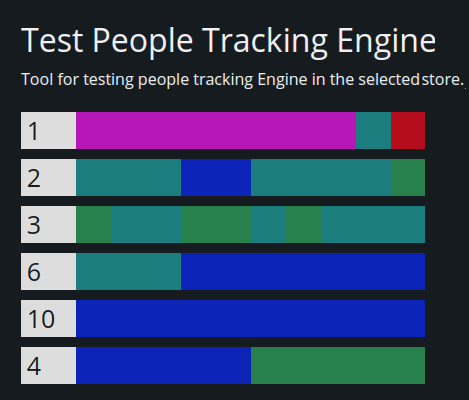
\includegraphics[scale=.80]{./Figures/simsWebApp2.png}
	\caption{Interacción de las personas con cada zona dibujada de interés.}
	\label{fig:simsWebApp2}
\end{figure}

\newpage

La aplicación web también arroja métricas sobre el recinto. Ofrece en una tabla cuales fueron las zonas más transitadas o más populares como también el mapa de calor del recinto (por donde caminaron las personas), como se puede observar en las figuras \ref{fig:metricasWebApp} y \ref{fig:metricasWebApp2} respectivamente.

\begin{figure}[ht]
	\centering
	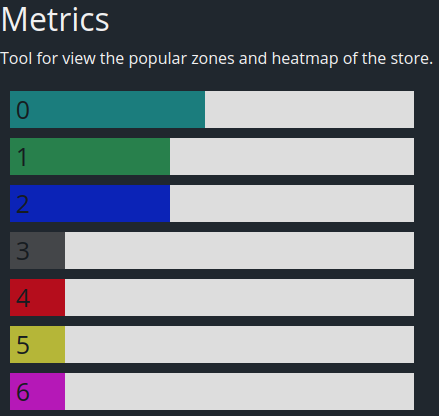
\includegraphics[scale=.80]{./Figures/metricasWebApp.png}
	\caption{Métricas de las zonas de interés del recinto.}
	\label{fig:metricasWebApp}
\end{figure}

\begin{figure}[ht]
	\centering
	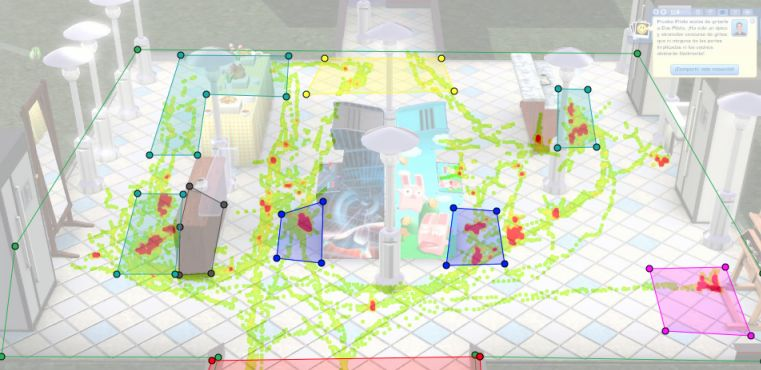
\includegraphics[scale=.70]{./Figures/metricasWebApp2.jpg}
	\caption{Mapa de calor del recinto.}
	\label{fig:metricasWebApp2}
\end{figure}

\newpage

De los resultados obtenidos se puede llegar a la conclusión que las zonas más visitadas del recinto son las zonas de comida y bebida (color cyan) y las zonas de juegos (color azul). 
% Chapter Template

\chapter{Conclusiones} % Main chapter title

\label{Chapter5} % Change X to a consecutive number; for referencing this chapter elsewhere, use \ref{ChapterX}


%----------------------------------------------------------------------------------------

%----------------------------------------------------------------------------------------
%	SECTION 1
%----------------------------------------------------------------------------------------

\section{Resultados obtenidos}

Se desarrolló e implementó con éxito un sistema de monitoreo de personas aplicando conocimientos adquiridos a lo largo de la carrera. Se alcanzó a cumplir el objetivo propuesto, el cual consistía en estudiar los movimientos que realiza una persona al ingresar y transitar un espacio durante al menos el 80\% del tiempo que la persona permanece en el espacio.

A continuación se listan los logros destacados del trabajo final:
\begin{itemize}
\item Cumplir con la planificación original.
\item Alcanzar las métricas pautadas para el sistema de seguimiento.
\item Entrar un modelo propio basado en OsNet.
\item Combinar técnicas de aprendizaje profundo con técnicas de aprendizaje automático para re-identificación de personas.
\item Re-identificar a las personas que salen de cámara o son ocluidas durante un tiempo considerable.
\item Generar material en video simulado para ensayar el sistema.
\end{itemize}


A continuación se resaltan aquellas materias de mayor relevancia para este trabajo:
\begin{itemize}
\item Gestión de Proyectos: la elaboración de un plan de proyecto para organizar el trabajo final, facilitó la realización del mismo y evitó demoras innecesarias.
\item Análisis de datos: el análisis de los datos de entrenamiento y su preprocesamiento permitieron mejorar los resultados de entrenamiento.
\item Aprendizaje automático: el uso de técnicas de segmentación y clasificación para la re-identificación de personas.
\item Visión por computadora I y II: la experiencia adquirida en el uso de algoritmos y modelos de detección de objetos fueron vitales para la realización de este trabajo.
\end{itemize}

%----------------------------------------------------------------------------------------
%	SECTION 2
%----------------------------------------------------------------------------------------
\section{Trabajo futuro}

Utilizando la experiencia adquirida en la realización de este trabajo se encontraron diferentes aspectos de mejora del prototipo, necesarios para que se convierta en un producto comerciable:

\begin{itemize}
\item Mejorar el modelo entrenado de OsNet utilizando \textit{triple-loss} y datos de diferentes orígenes.
\item Evaluar la utilización de \textit{Tensorflow Real Time} para mejorar los tiempos de cómputo de los modelos de IA.
\item Evaluar que tipo de dispositivo podría ejecutar el sistema completo en tiempo real.
\item Evaluar el uso de cámaras de mayor ángulo visual para capturar más espacio del recinto.
\item Evaluar incorporar modelos de detección de pose a fin de obtener más información de la actividad que desarrollada la persona en el recinto.
\end{itemize}

Durante la utilización de la interfaz del sistema también se encontraron aspectos a mejorar en cuanto a la usabilidad:
\begin{itemize}
\item Crear una base de datos para almacenar las métricas obtenidas en cada ensayo o ejecución.
\item Disponer de la posibilidad de visualizar varias cámaras o recintos desde la misma interfaz.
\item Desarrollar una interfaz reducida para su visualización en dispositivos móviles.
\item Elaborar alertas programables relativas a que está sucediendo en el local.
\end{itemize}
 

%----------------------------------------------------------------------------------------
%	CONTENIDO DE LA MEMORIA  - APÉNDICES
%----------------------------------------------------------------------------------------

\appendix % indicativo para indicarle a LaTeX los siguientes "capítulos" son apéndices

% Incluir los apéndices de la memoria como archivos separadas desde la carpeta Appendices
% Descomentar las líneas a medida que se escriben los apéndices

%\include{Appendices/AppendixA}
%\include{Appendices/AppendixB}
%\include{Appendices/AppendixC}

%----------------------------------------------------------------------------------------
%	BIBLIOGRAPHY
%----------------------------------------------------------------------------------------

\Urlmuskip=0mu plus 1mu\relax
\raggedright
\printbibliography[heading=bibintoc]

%----------------------------------------------------------------------------------------

\end{document}  
